\chapter{Radio neutrino detection}
Neutrinos on their own aren't detectable, unlike say protons we can't expect
them to produce Brehmsstrallung or any other kind of directly observable
radiation as they aren't charged and thus don't couple to photons. We'll need
to convert them to charged particles first which then can generate some kind of
detectable signal.  

To this end we'll need a big volume in which they can interact to produce
charged particles, we'll be choosing ice for this.  Even though there are a lot
of volumes such as the water or rock the ice has a few particular properties
which make it more usable:
\begin{itemize}
  \item contrary to some kind of sediment, ice is mostly see-through for electromagnetic radiation but it's still possible
    to differentiate between neutrino signals and other particles
  \item contrary to water as a medium which is used e.g in the Super-Kamiokande detector\cite{SuperKamio}, ice
    was naturally formed and it isn't needed to construct some kind of dome
\end{itemize}
\section{Neutrino interactions in ice}
As neutrinos propagate through ice they can interact weakly with the nuclei.
The main mechanisms of interaction is via charged- and neutral
currents\cite{NuRadioMc} as is also depicted in figure
\ref{fig:NeutrinoNucleusInteraction}.
\begin{figure}[h!]
	\begin{minipage}{\textwidth}
		\begin{minipage}{0.49\textwidth}
			\centering
			\begin{tikzpicture}
				\begin{feynman}
					\vertex (a0) {quark};
					\vertex[above=0.5cm of a0] (a1) {quark};
					\vertex[above=0.5cm of a1] (a2) {quark};
					\vertex[right=2cm of a0] (b0) {quark};
					\vertex[right=2cm of a1] (b1) {quark};
					\vertex[right=2cm of a2] (b2) {quark};
					\vertex[right=1.0cm of a2] (am);
					\vertex[above=1cm of am] (c0);
					\vertex[above=1cm of c0] (c1);
					\vertex[above=1cm of c1] (cm);
					\vertex[left=1cm of cm] (a3) {$\nu_l$};
					\vertex[right=1cm of cm] (b3) {$l$};
					\diagram* {
						{[edges=fermion]
							(a0) -- (b0)
						},
						{[edges=fermion]
							(a1) -- (b1)
						},
						{[edges=fermion]
							(a2) -- (c0) -- (b2)
						},
						{[edges=fermion]
							(a3) -- (c1) -- (b3)
						},
						{[edges=boson, edge label=W]
							(c0) -- (c1)
						},
					};
				\end{feynman}
			\end{tikzpicture}
		\end{minipage}
		\begin{minipage}{0.49\textwidth}
			\centering
			\begin{tikzpicture}
				\begin{feynman}
					\vertex (a0) {quark};
					\vertex[above=0.5cm of a0] (a1) {quark};
					\vertex[above=0.5cm of a1] (a2) {quark};
					\vertex[right=2cm of a0] (b0) {quark};
					\vertex[right=2cm of a1] (b1) {quark};
					\vertex[right=2cm of a2] (b2) {quark};
					\vertex[right=1.0cm of a2] (am);
					\vertex[above=1cm of am] (c0);
					\vertex[above=1cm of c0] (c1);
					\vertex[above=1cm of c1] (cm);
					\vertex[left=1cm of cm] (a3) {$\nu$};
					\vertex[right=1cm of cm] (b3) {$\nu$};
					\diagram* {
						{[edges=fermion]
							(a0) -- (b0)
						},
						{[edges=fermion]
							(a1) -- (b1)
						},
						{[edges=fermion]
							(a2) -- (c0) -- (b2)
						},
						{[edges=fermion]
							(a3) -- (c1) -- (b3)
						},
						{[edges=boson, edge label=Z]
							(c0) -- (c1)
						},
					};
				\end{feynman}
			\end{tikzpicture}
		\end{minipage}
	\end{minipage}
	\caption{Most prominent ways of neutrino-nucleus interaction}
	\label{fig:NeutrinoNucleusInteraction}
\end{figure}\\
With the produced leptons in the W boson mediated interaction being either electrons,
resulting in an electromagnetic shower, muons which typically go undetected as they live
too long or
tauons which will decay via
\begin{equation}
	\tau^- \rightarrow e^- + \bar{\nu}_e + \nu_\tau
\end{equation}
or, less ideally
\begin{equation}
	\tau^- \rightarrow \mu^- + \bar{\nu}_\mu + \nu_\tau
\end{equation}
In both of the possible interactions (W or Z exchange) the resulting nucleus
will result in an hadronic shower, for the neutral current interaction (mediated
by the Z boson) the fraction of the neutrino energy that gets transferred to
the nucleon is described by the inelasticity $y$ and is heavily shifted towards
small values of $y$\cite{elasticity_y}. This causes a big, irreducible
uncertainty when trying to estimate the original neutrino energy from these
kinds of events.  With the charged current interaction (mediated by the $W^\pm$
bosons) this isn't a problem however as the full neutrino energy ends up in the
resulting cascades.
\section{Askaryan effect}
\label{sec:Askaryan}
For a particle shower to emit strong radio signals, two conditions have to be met:
\begin{itemize}
	\item There needs to be a separation of positive and negative charges in the shower front 
	\item The signals produced over the length of the shower profile need to overlap coherently.
\end{itemize}
The \textit{Askaryan} \cite{Askaryan} effect, which is responsible for the
production of Askaryan radiation describes the effect at radio frequencies
which abides by both of these conditions.  In general it's a quite difficult
effect but we'll give a crude overview.  The previously described interactions
of the neutrinos with nuclei create a shower of secondary charged particles
containing a charge anisotropy.  This charge imbalance is a result of medium
electrons either Compton scattering into the advancing shower or annihilating
with shower positrons.  In the end you have a moving charge anisotropy,
propagating faster than the speed of light in the medium, creating Cherenkov
radiation.  

Cherenkov radiation is like the electromagnetic equivalent of a sonic boom, a
sonic boom happens when something goes faster than the speed of sound in the
medium; A particle emits Cherenkov radiation if it goes faster than the speed
of light in the medium.  Choosing the particle trajectory to lie along the z
axis an approximate equation can be found\cite{jackson1998classical} for
$\frac{\text{d}^2 \mathscr{J}}{\text{d}\omega \text{d}\Omega}$, which is the energy
radiated per elementary unit solid angle and per elementary unit frequency
interval:
\begin{equation}
	\frac{\text{d}^2 \mathscr{J}(\omega)}{\text{d} \omega \text{d} \Omega} = \frac{q^2}{4\pi}\sqrt{\frac{\mu}{\epsilon}}\beta^2\omega^2\delta^2[\omega(1-\beta \mathbf{e}_r\cdot\mathbf{e}_z)]|\mathbf{e}_r\times\mathbf{e}_z|^2 \label{equation: 4.128 in elektromagnetisme}
\end{equation}
Now we can re-write this equation in spherical coordinates, which gives $1-\beta \mathbf{e}_r\cdot\mathbf{e}_z = 1-\beta\cos(\theta_c)$ in the delta function. We thus only expect radiation if
\begin{equation}
\cos(\theta_c) = \frac{1}{\beta} = \frac{c'}{u} = \frac{c}{n}\cdot\frac{1}{u}
\end{equation}
With u the local speed of light in the medium and n the index of refraction, an optical
property of a medium which we'll later on thoroughly discuss.
If $u>\frac{c}{n}$, Cherenkov radiation will
be emitted along a cone surface with half angle $\frac{\pi}{2}-\theta_c$ as
illustrated in figure \ref{figure: Cherenkov illustratie}. Integrating equation
\ref{equation: 4.128 in elektromagnetisme} over the solid angle and formally
dividing by the time interval we get:
\begin{equation}
	\frac{\text{d}^2\mathscr{J}}{\text{d}\omega \text{d}t} = \frac{q^2}{4\pi}\sqrt{\frac{\mu}{\epsilon}}\beta\omega\left(1-\frac{1}{\beta^2}\right)	
\end{equation}
We see that the energy is proportional to $\omega$, so we expect that most
radiation will be emitted "in blue" with a cut-off frequency above which the
equation $\cos\theta = 1/(n\beta)$ can no longer be satisfied, this "in blue"
characteristic is responsible for the blue glow seen in nuclear reactors as
seen in figure \ref{figure: Cherenkov reactor} .  For ice the index of
refraction is roughly 1.78 in deep ice, so we expect an ultra-relativistic
particle to produce the most radiation at around 56° opening as 
\begin{equation}
	\cos(\theta_c) \approx \frac{1}{n} \implies \cos^{-1}\left(\frac{1}{1.78}\right)\approx 56\text{°}
\end{equation}
\begin{figure}
\centering
\begin{minipage}{0.45\textwidth}
	\centering
	\copyrightbox[r]{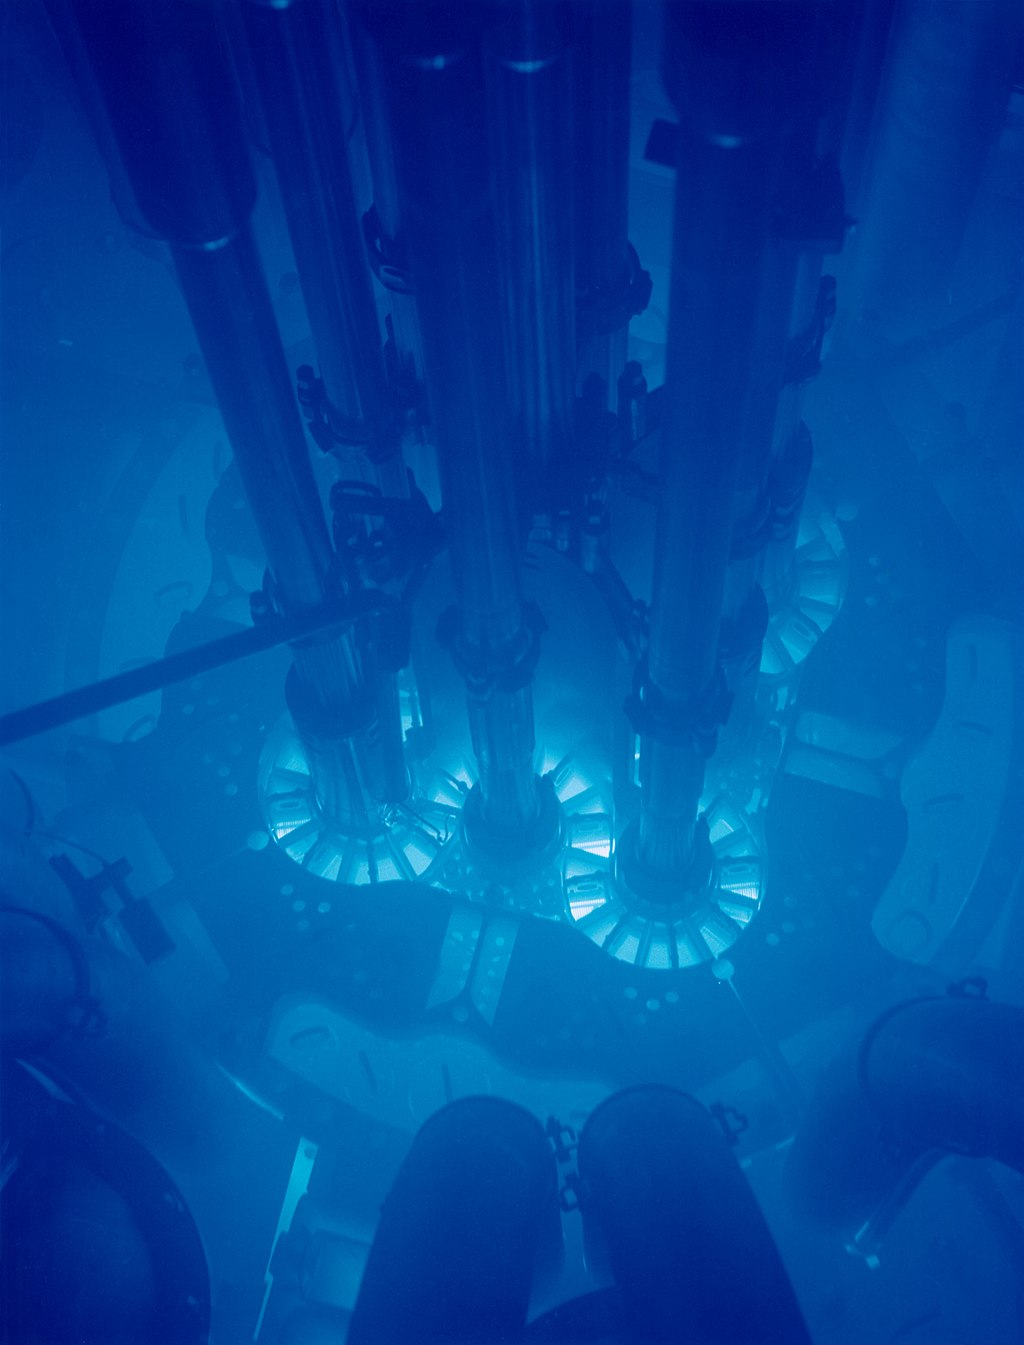
\includegraphics[height = 0.8\textwidth]{Cherenkov-reactor.jpg}}{\textcopyright Argonne National Laboratory\\Advanced Test Reactor core, Idaho National Laboratory}
	\caption{Cherenkov radiation in a nuclear reactor}
	\label{figure: Cherenkov reactor}
\end{minipage}
\hspace{0.05\textwidth}
\begin{minipage}{0.45\textwidth}
	\centering
	\copyrightbox[r]{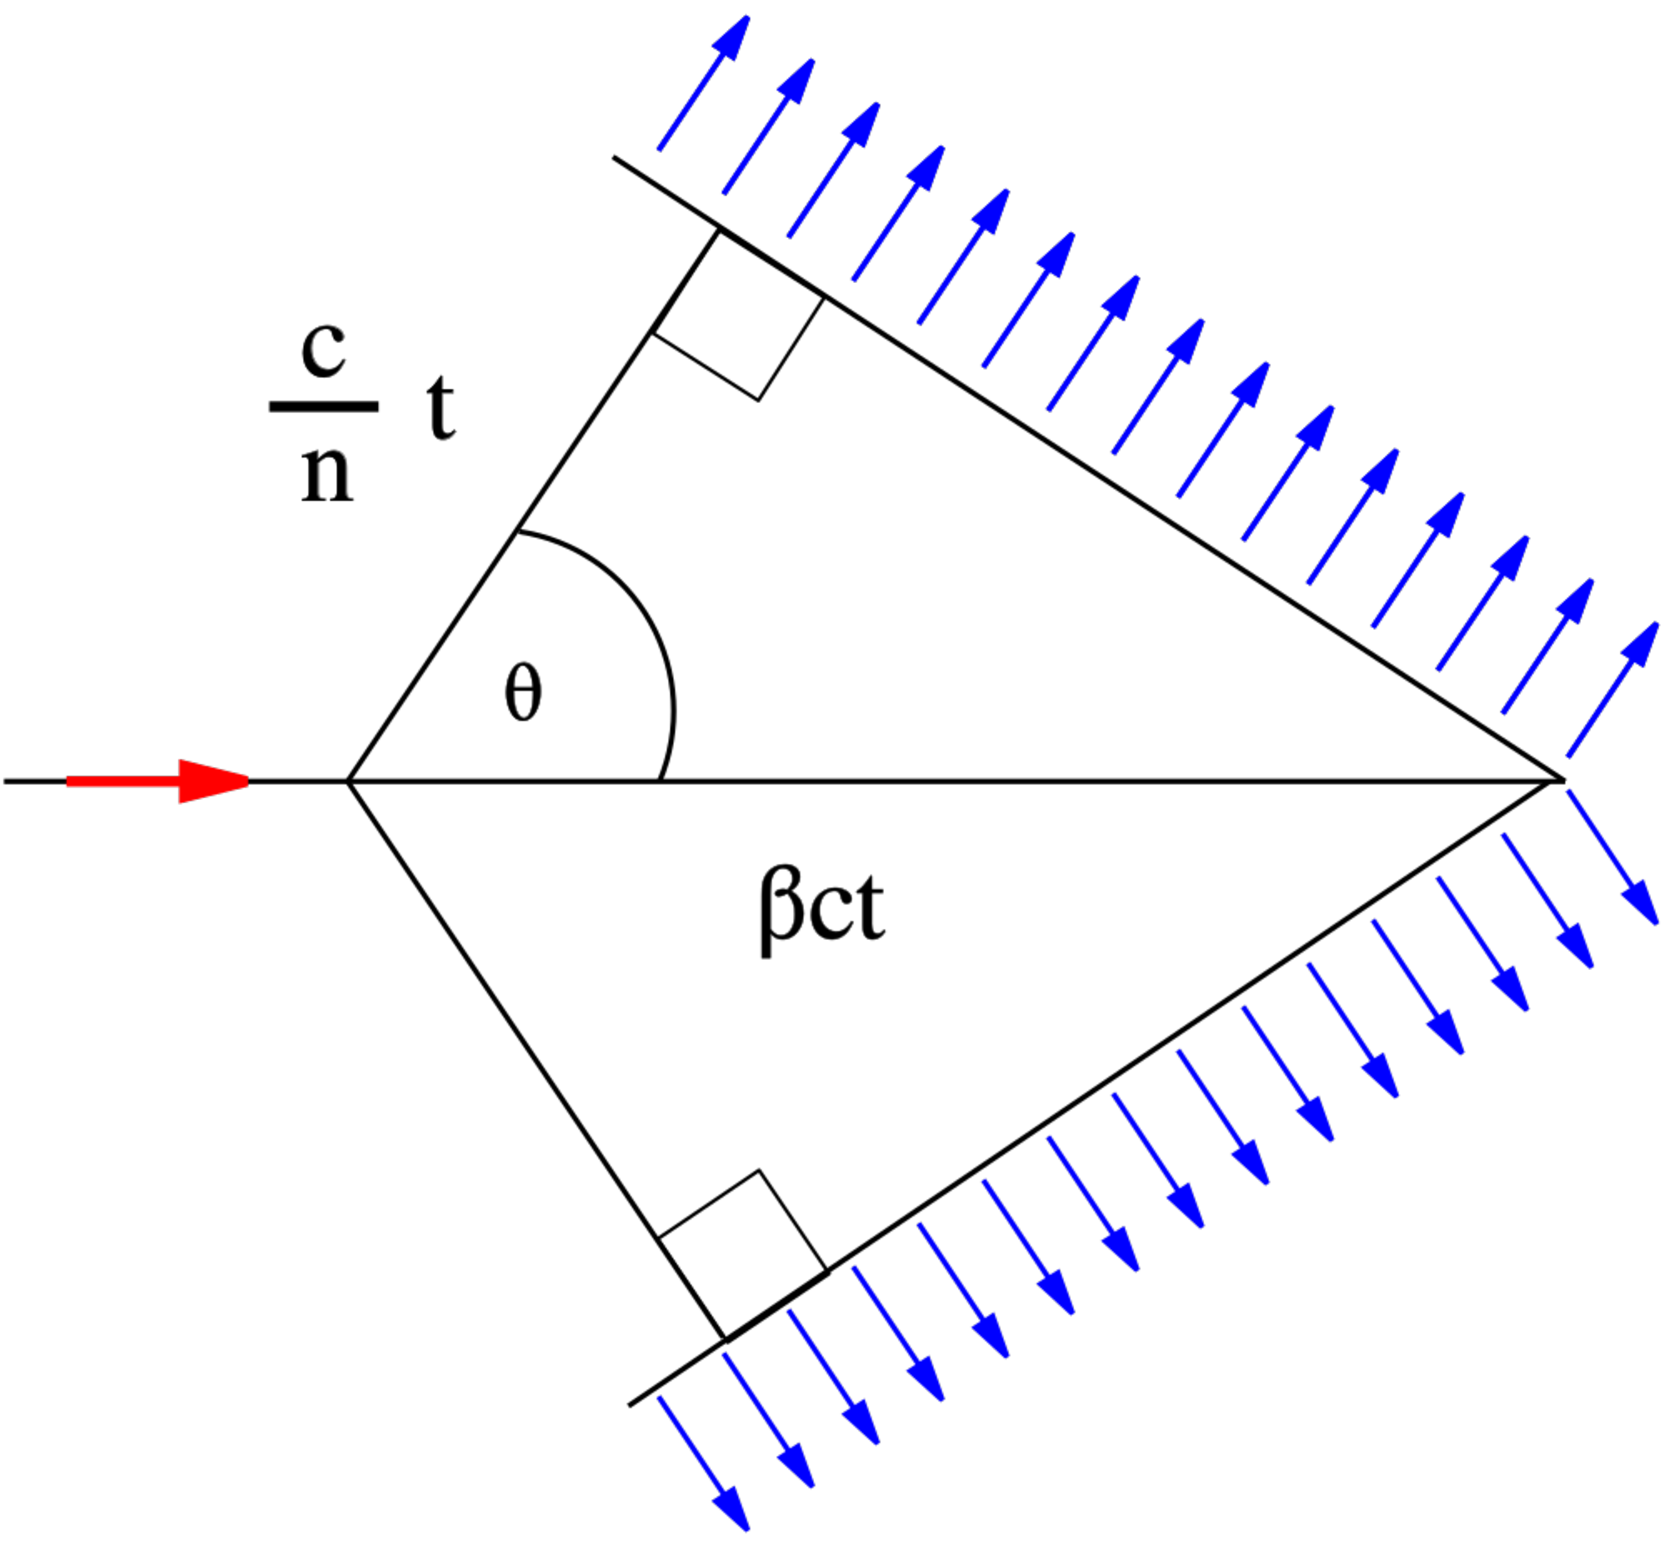
\includegraphics[height = 0.8\textwidth]{Cherenkov.pdf}}{\textcopyright Arpad Horvath}
	\caption{Diagrammatic representation of Cherenkov radiation}
	\label{figure: Cherenkov illustratie}
\end{minipage}
\end{figure}
Of course this is just an estimate, as the actual index of refraction is depth-dependent which
we'll get to in section \ref{section:Ice Model}.
Now this explains how the signals get generated but logically, from only knowing this
we'd expect radio waves to almost be non-existent 
due to the "in blue" nature of Cherenkov radiation. 

To understand why this isn't the case we'll need another piece of the puzzle: coherent overlap.
Coherent overlap in the radio wave spectrum range can be intuitively explained as
follows: generally the shower is of length
$\mathcal{O}$(10cm)\cite{Huege_2017}, over this length the radiation gets
emitted, most frequencies decoherently interfering, but radio waves with wavelengths of 
$\approx$ 10cm coherently interfere, and it's these waves we then wish to detect.
The radiation generated trough this Askaryan effect is called \textit{Askaryan radiation}.

The Askaryan radiation is polarized perpendicular to the
Cherenkov cone, this can be useful to discern between different Cherenkov cones whom,
timely, would generate the same response. This concept is illustrated below in 2D where
two neutrinos from different directions would generate the same signal in the detector.

\begin{figure}[h!]
	\centering
	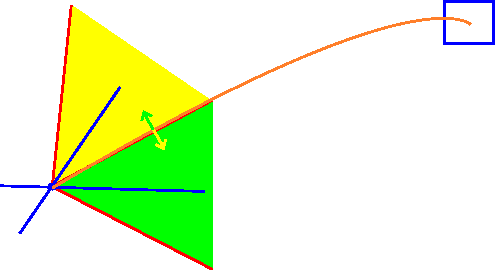
\includegraphics[width=0.5\textwidth]{illu_polarization.pdf}
\end{figure}

If the detector has a way to differentiate between polarization however, there would be no
doubt where the neutrino originated from as the one producing the yellow Cherenkov cone
would have a downwards polarization and the one producing a green Cherenkov cone would have
an upwards polarization, note that in 3D infinite different Cherenkov cones could generate
the same timely signal (think of rotating the cone around a line on the cone) so both vertical
and horizontal polarization information is needed.


\section{RNO-G}
Both cosmic ray and neutrino detectors face the same main problem at the
highest energies: the steeply falling flux (as was previously seen in figure
\ref{figure:Neutrino fluxes}) requires large effective areas, which leads to
the construction of neutrino detectors with volumes on the cubic kilometer
scale like IceCube\cite{IceCubeTechnical} which works on the principle of
detection neutrinos with visible light.  But even IceCube has it's limitations,
it's still too small to observe neutrino events above the 10 PeV
scale\cite{IceCubeGen2}, that's why a new detector was needed which was even
bigger and able to observe cosmogenic neutrinos.  We could just make IceCube
bigger but this would cost a lot of money as the individual detectors need to
be spaced closely as the attenuation length is quite short for light in the
visible spectrum propagating through ice.  

The proposed solution was to work with radio wave detectors, leveraging the
previously discussed Askaryan effect (see section \ref{sec:Askaryan}).  Besides
the advantage radio waves have due to their abundance, they can also propagate
way further in ice than visible light making it possible to space the
individual detectors further apart. The proposed location was Greenland, an
island country in North America and part of the Kingdom of Denmark which has
large ice sheets.
\begin{figure}
  \centering
  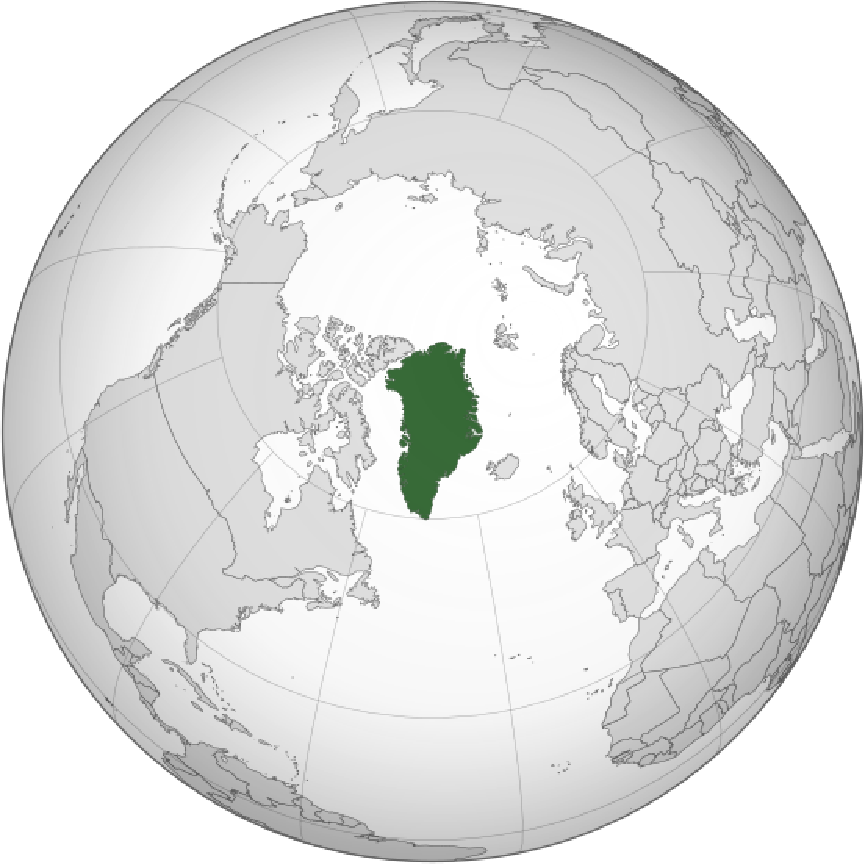
\includegraphics[width=0.5\textwidth]{figures/GreenlandOP.pdf}
  \caption{orthographic projection of Greenland with the red star representing the approximate RNO-G location}
  \label{fig:GreenlandOP}
\end{figure}
The proposal for RNO-G, which was later funded and now in the construction
phase, is for it to be an array of autonomous radio stations each of which having both
surface channels and various deep channels resulting in a total of 24 channels
per station. The whole project builds heavily on the knowledge obtained through
previous radio based neutrino detectors like the NuMoon\cite{numoon} project,
ANITA\cite{ANITA}, ARA\cite{ARA},ARIANNA\cite{Barwick_2015} and RICE\cite{RICE}.
\subsection{Hardware}
One such detector is illustrated in figure \ref{fig:detector}, the plan is to
build 35 of these as is shown in figure \ref{fig:station map}\footnote{note
that all the individual detectors are numbered but also named after various species living in
Greenland (in the native tongue)}. Looking closely at one such detector we see
just below the surface 9 Log Periodic Dipole Antennas (LPDAs), these are used
to detect air shower muon signals as muons will also generate Cherenkov
radiation in the ice whose signals can then be filtered out.  Aside form these
surface detectors there are also deep components of the detector which can be
split up in three parts: Two \textit{helper strings} and the \textit{power
string}.

The helper strings are the 2 vertical cables shown on the right of figure
\ref{fig:detector} each housing 2 vertically polarized antennas (Vpols), one
quadslot antenna for the horizontal polarization component (Hpol) and one radio
pulser on each helper string which can be used to generate calibration signals.
As was previously mentioned the polarization can be used to
distinguish between possible Cherenkov cones generating the same resulting
pulse, that's why both the helper and power string are equipped with both kinds
of polarized antennae.

The power string (the leftmost vertical cable) is more densely instrumented
than the helper strings: At the bottom it houses a set of four Vpol and two
Hpol antennas with a spacing of 1m called the \textit{phased array}, arguably
the most important channels in a station as it's spaced closely together and
can thus use the principle of phasing the channels to get higher precision.
Further up the string, with a spacing of 20m, are three more Vpol antennas.
\begin{figure}
  \centering
  \copyrightbox[r]{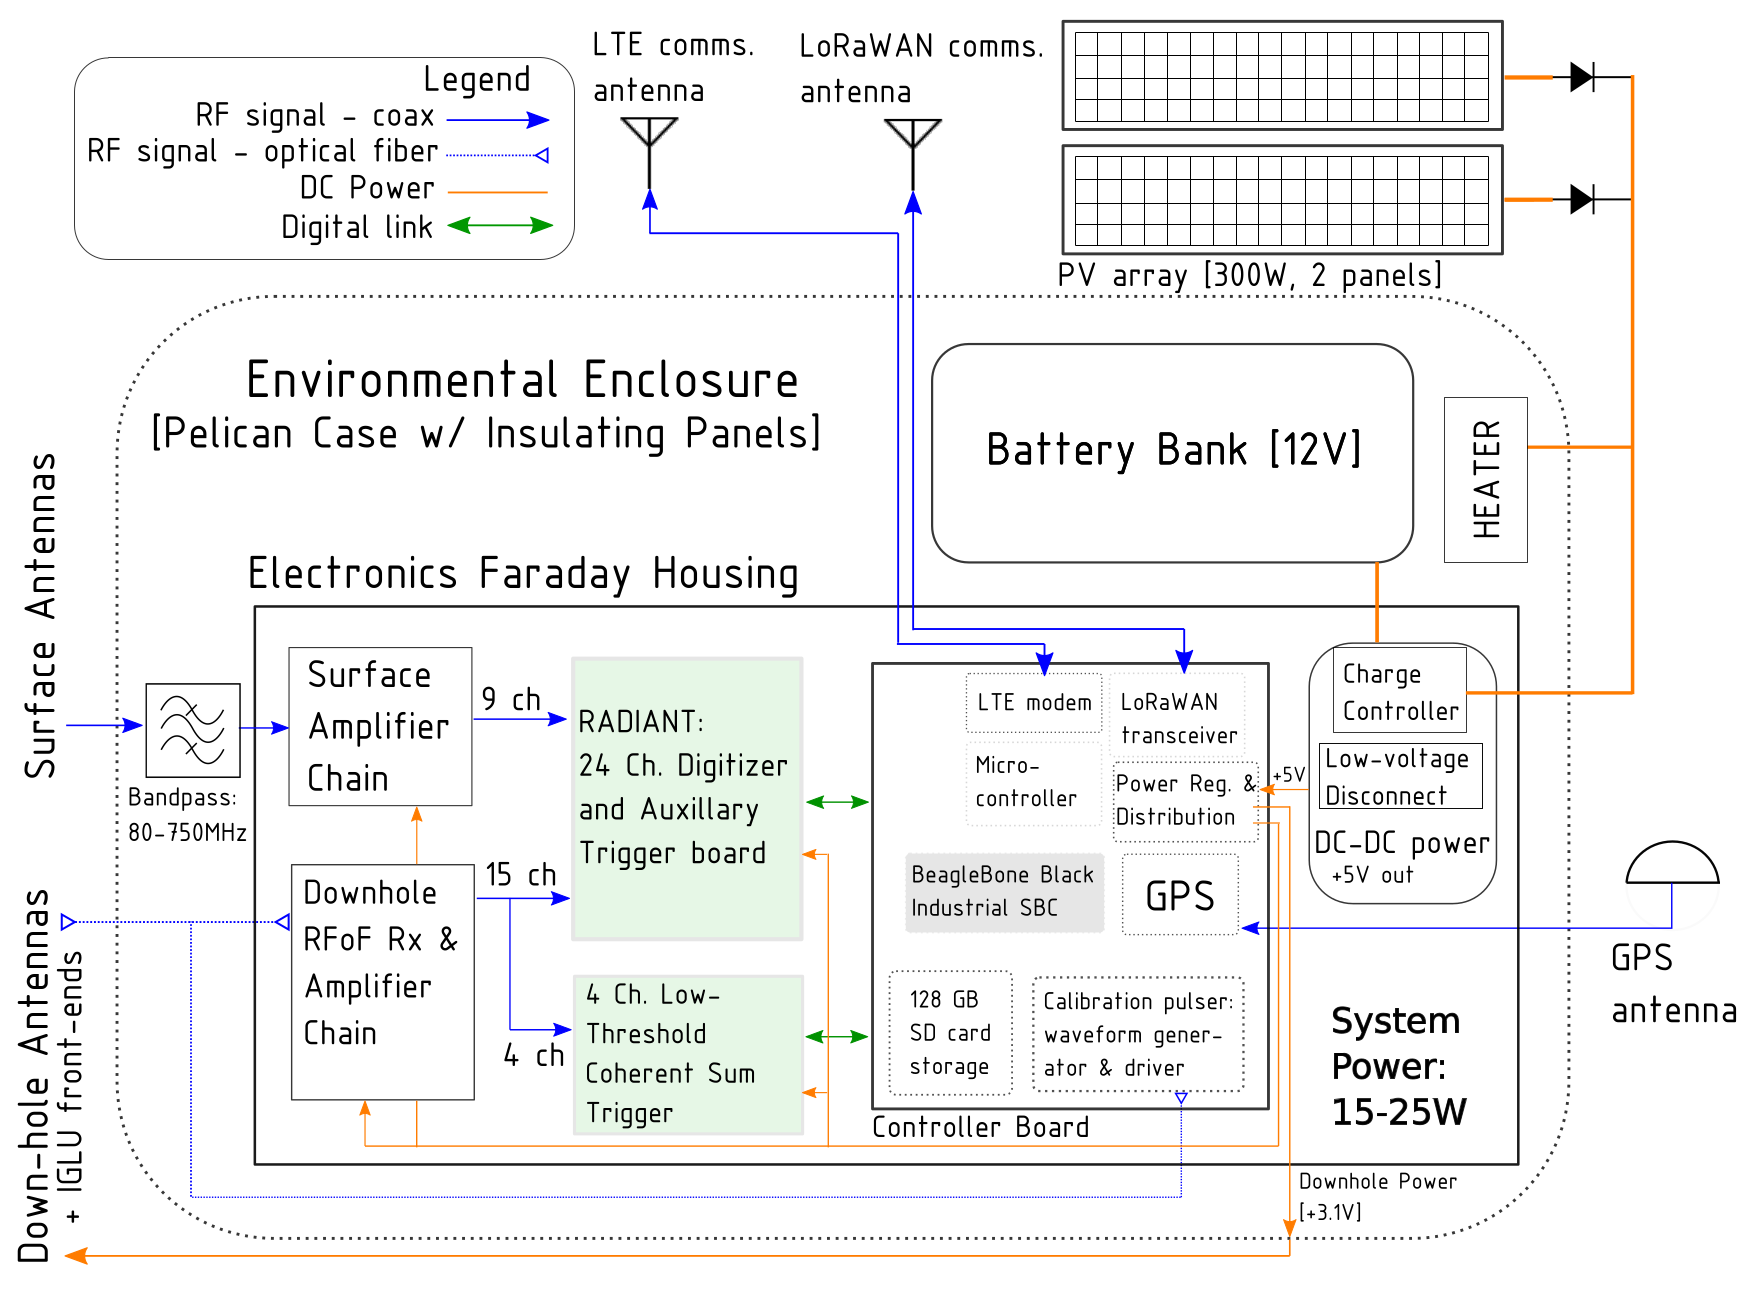
\includegraphics[width=0.85\textwidth]{SysDiagRNOG.png}}{\textcopyright Design and Sensitivity of the Radio Neutrino Observatory in Greenland (RNO-G) by J.A. Aguilar et. al}
  \caption{System diagram for a RNO-G station}
  \label{fig:SysDiag}
\end{figure}

A full system diagram for a RNO-G station is shown in figure \ref{fig:SysDiag}, I'll
give a walk trough of how data gets collected.
The signal from each of the deep antennae are fed into a low-noise amplifier
directly above it, from there the signal is send to the data acquisition (DAQ)
system at the surface via a Radio Frequency over Fiber (RFoF) cable.  The
signals coming from the surface antennae are first passed through a Bandpass
filter of 80-750MHz\footnote{i.e a filter that only lets frequencies in this
range pass} prior to both them and the deep component signal ending up in the
RAdio DIgitizer and Auxiliary Neutrino Trigger (RADIANT), there it's again
amplified, digitized and, if a trigger threshold is reached, saved onto an SD
card. This data is then transmitted via a Long Term Evolution (LTE)
telecommunications network to a local server\footnote{There is additionally a
Long Range Wide Area Network (LoRaWAN) antenna as backup in case of problems
with the LTE network}, from where it is sent via a satellite link.

As a power source, battery banks are used whom are charged via solar panels.
But as there is't enough light during the Greenland winters, there're plans to
build wind turbines (with one of the problems being the possibly detectable RF
noise the 'engine' would produce).

As was previously explained the radio signal from a neutrino often travels
along both direct and refracted paths, designated DnR, to the deep array (as shown
on figure \ref{fig:DnR}).
\begin{figure}
  \centering
  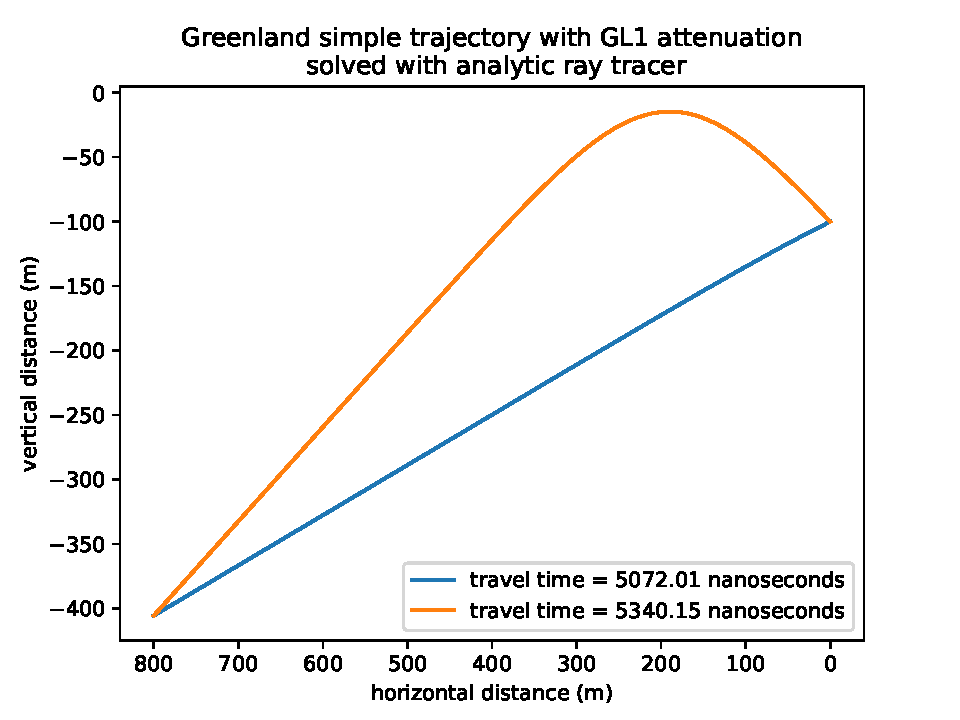
\includegraphics[width=0.5\textwidth]{DnR.pdf}
  \caption{example simulation showing both direct and refracted path from a neutrino vertex (bottom left) to a detector (top right)}
  \label{fig:DnR}
\end{figure}
This double pulse characteristic would be a smoking-gun signature of an in-ice
source. The two helper strings are needed for a full direction reconstruction.
Three independent measurements are needed for azimuthal information, which is
provided by the Vpol (Vertical polarization) antennas and placing the Hpol
(Horizontal polarization) antennas at different depths on every string, both
zenith and azimuth information will be provided for those signals. The helper
strings' calibration pulsers, as well as one on the surface, will ensure
regular monitoring of the performance of the station and provide information
useful for precise calibration of the antenna geometry.
\subsection{Reconstruction: Lookup tables}
The main simulation code we'll be using consists of 2 parts:
NuRadioMC\cite{Glaser_2020} and NuRadioReco\cite{Glaser_2019}. NuRadioMC uses
Monte Carlo simulations to generate neutrino events in the ice and simulates
how they propagate to the various channels, which will be covered more in-depth
in the next chapter. NuRadioReco is reconstruction software, it simulates how
the various detectors would respond to the detected radio waves. This simulation
software is needed as the plan is to simulate a lot of neutrino events and
record the detector responses in a giant database, then, when an actual neutrino
event occurs, we'll only have to look in the database and match the actual
detector response to the simulated detector responses, thus finding the origin.
\begin{figure}
	\centering
	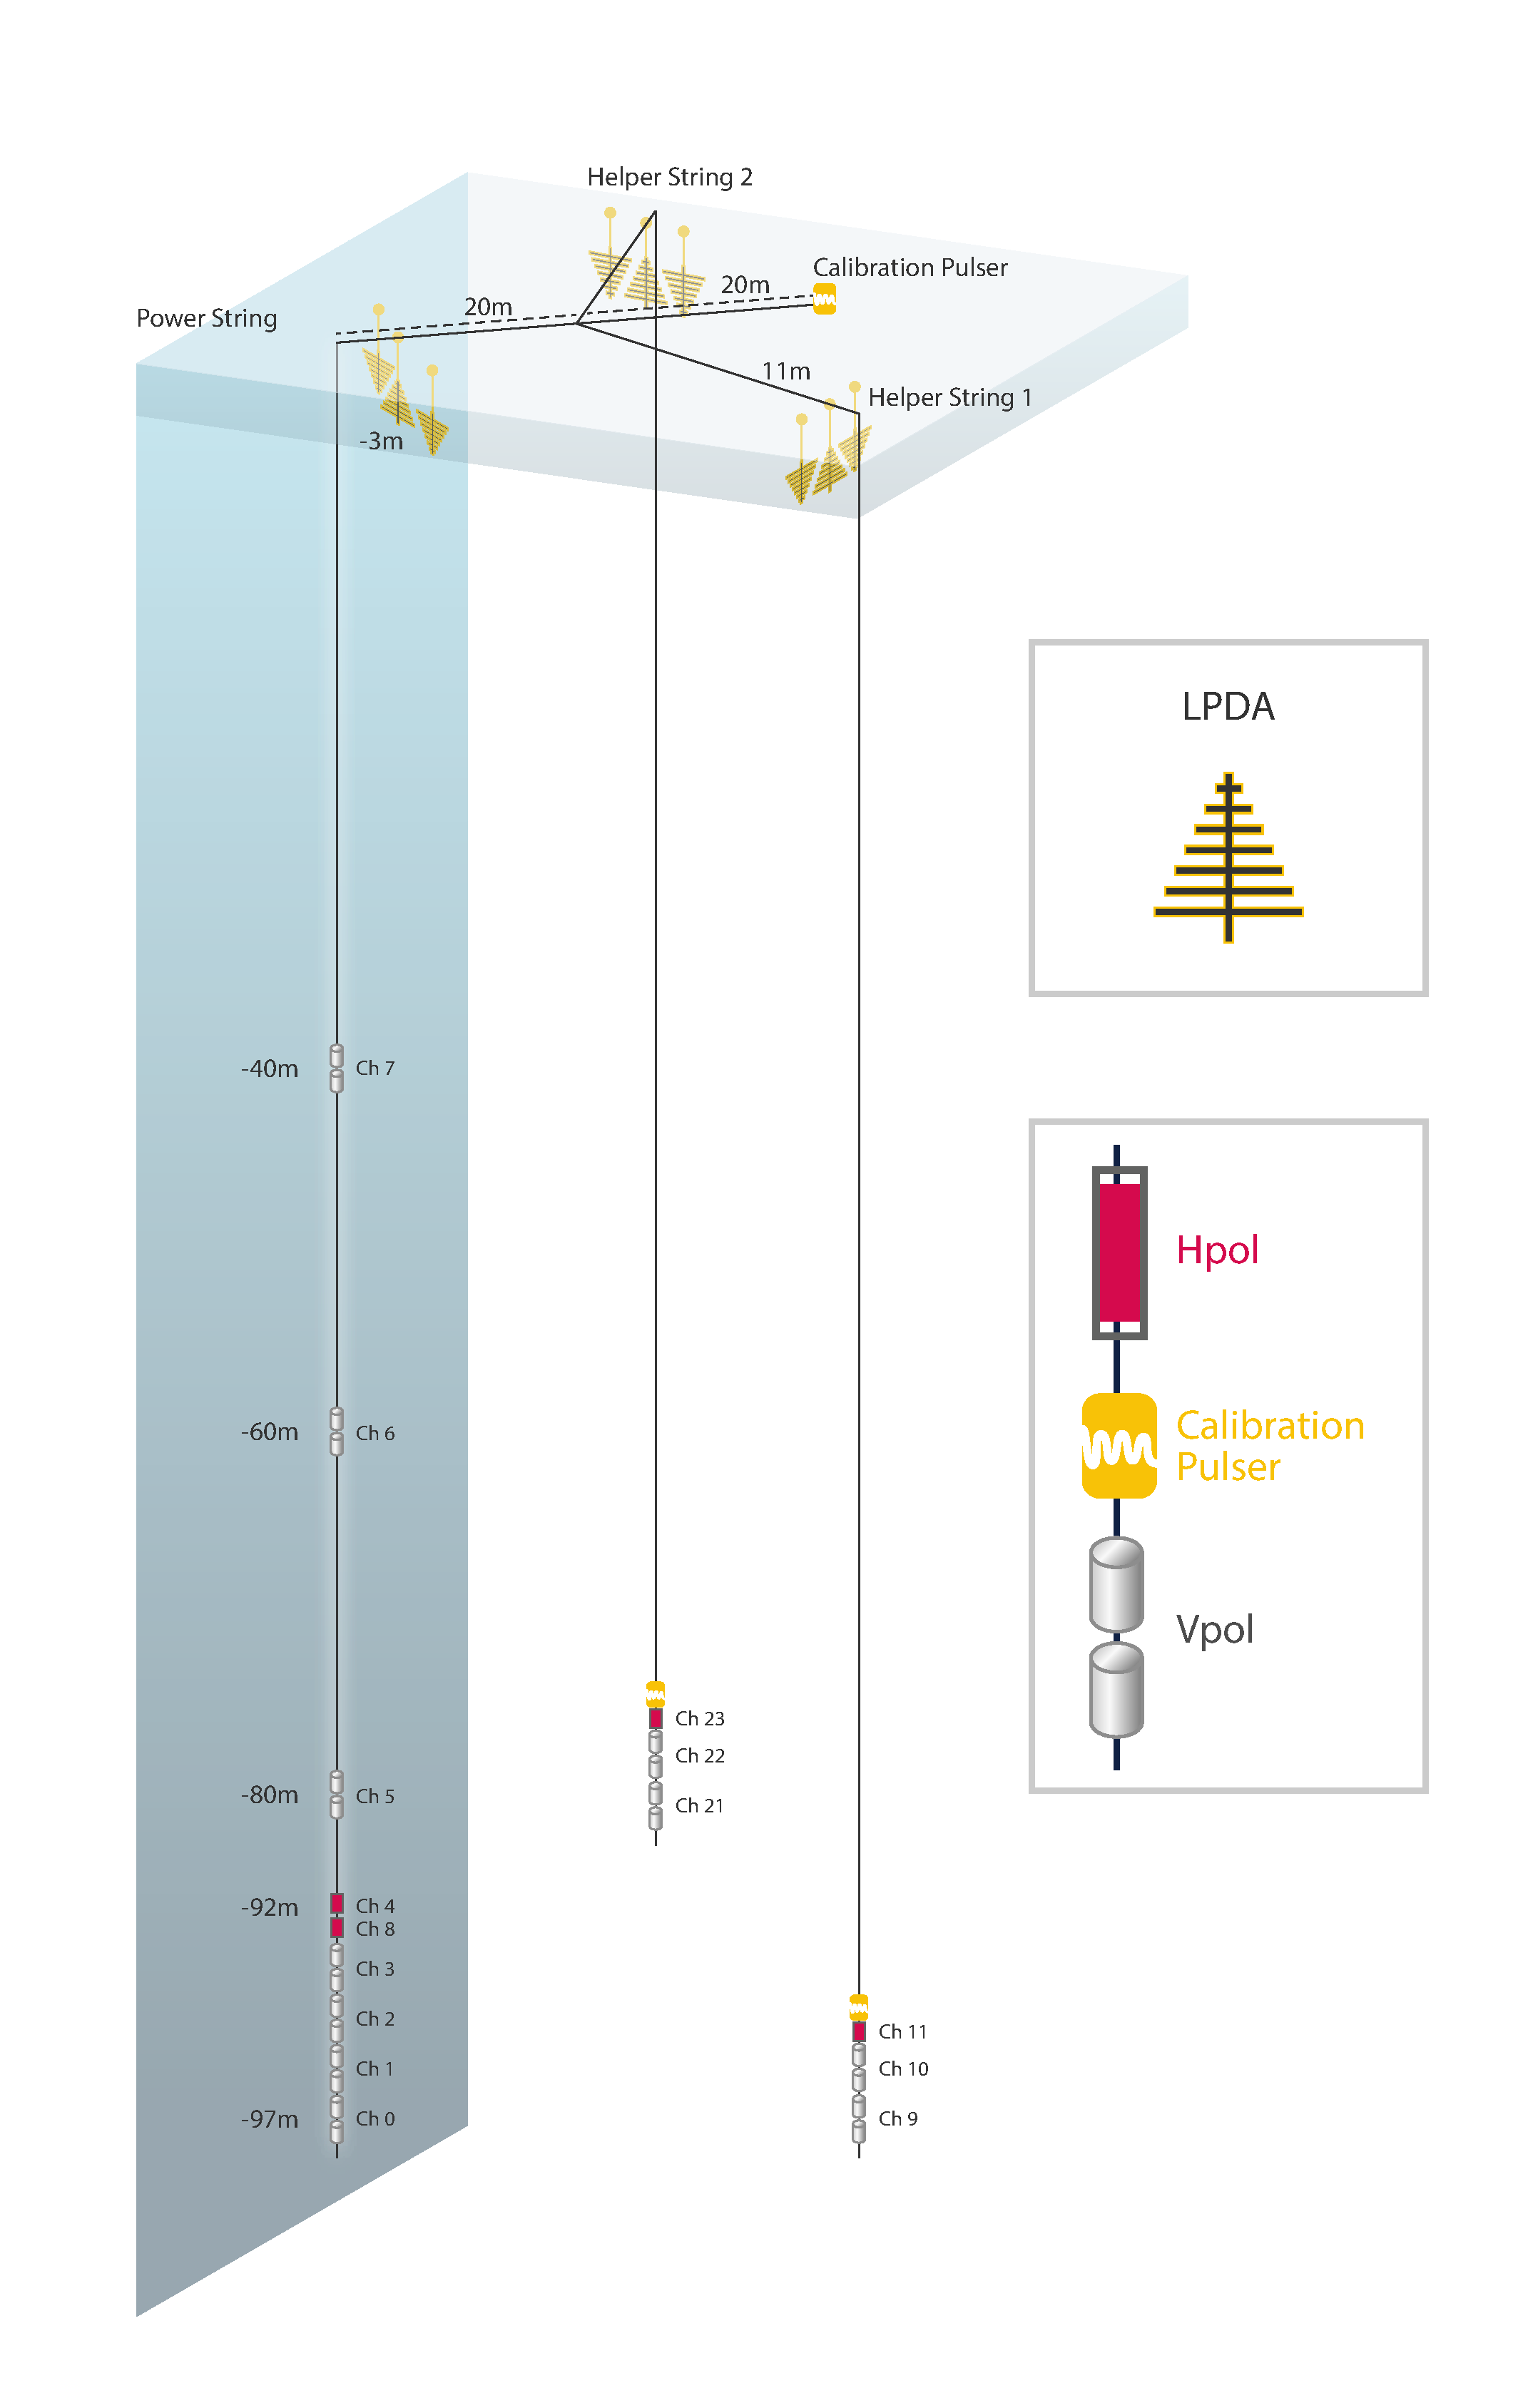
\includegraphics[height=0.9\textheight]{figures/detector.pdf}	
	\caption{diagram showing the numbering and locations of the various antennae}
	\label{fig:detector}
\end{figure}
\begin{figure}
	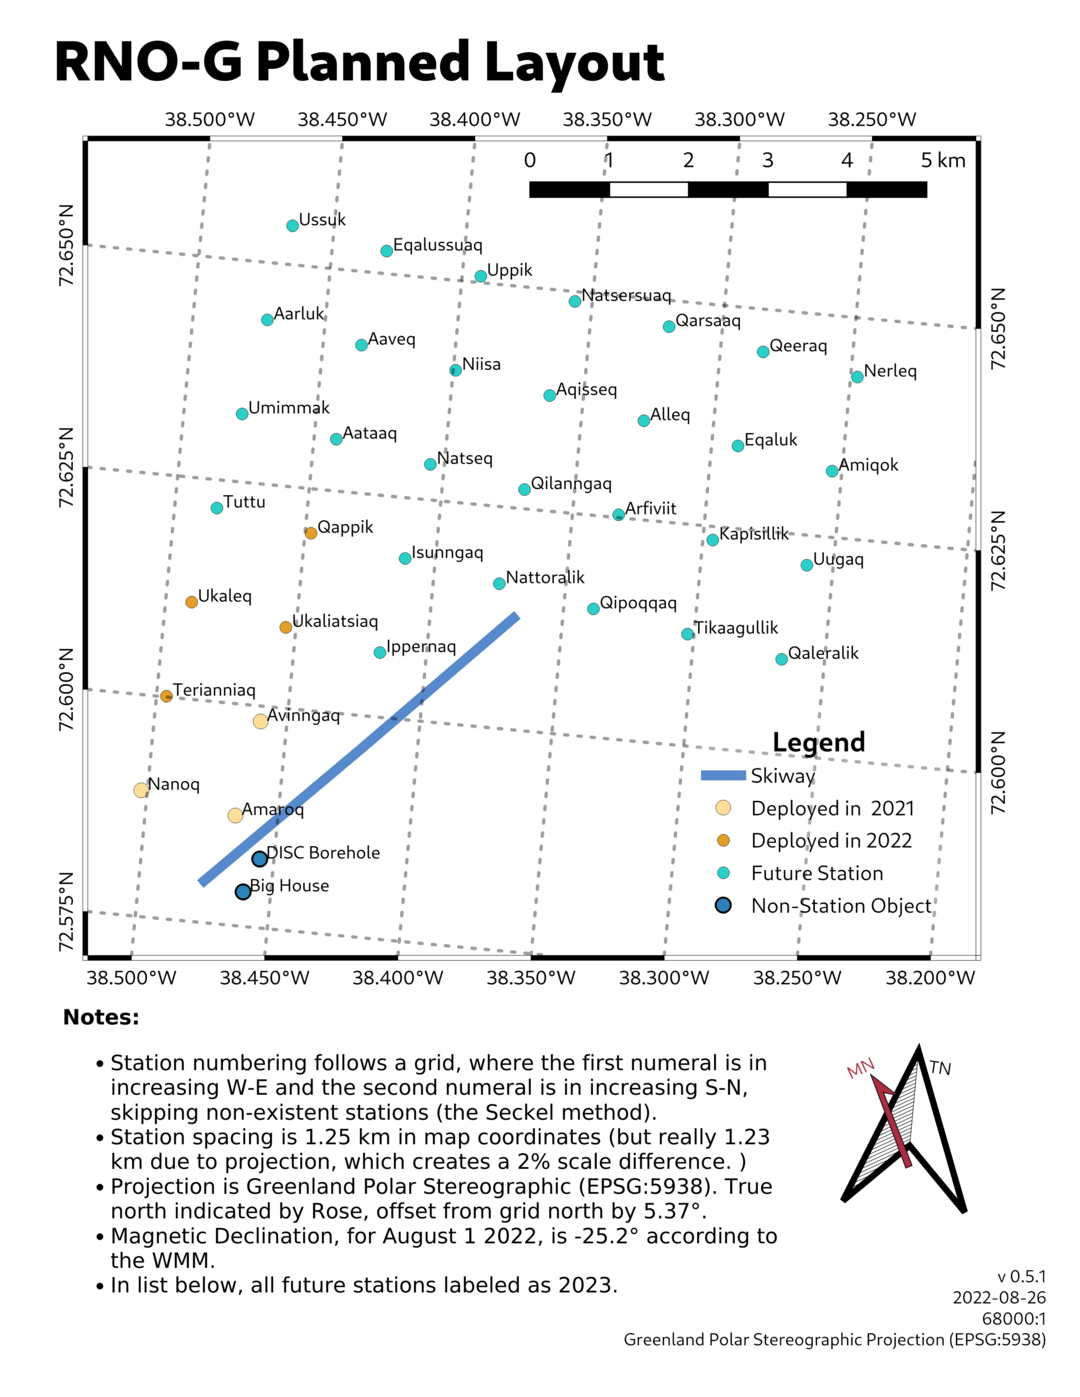
\includegraphics[width=\textwidth]{figures/station-map.png}	
	\caption{planned station layout}
	\label{fig:station map}
\end{figure}


